% !TeX root = ../main.tex

\chapter{模型建構}

本章為模型建構,在介紹完本文研究過程中所會使用到的理論與方法後,需要將這些理論與方法實際應用於模型中使用。這一章節將闡述各步驟中的建模流程以及收益分析中的等效模型與收益模型,並於下一章節進行案例分析。

\section{風力電場發電預測}

\subsection{時間序列預測建模流程}

自迴歸移動平均模型 $\text{ARIMA}(p, d, q)$ 的建模流程如圖 \ref{figure: Time Series Model Flow} 所示。在取得時間序列資料後,需要先進行平穩性檢驗,若時間序列不具備平穩性則必須差分 $d$ 次進行平穩化;接著繪製其 ACF 與 PACF 圖形並由其特徵初步決定其自迴歸項 $p$ 與移動平均項 $q$ 之值;初步階數選定之後透過 AIC 與 BIC 進行評價並選出最適模型以進行時間序列預測。

\begin{figure}[htbp]
  \centering
  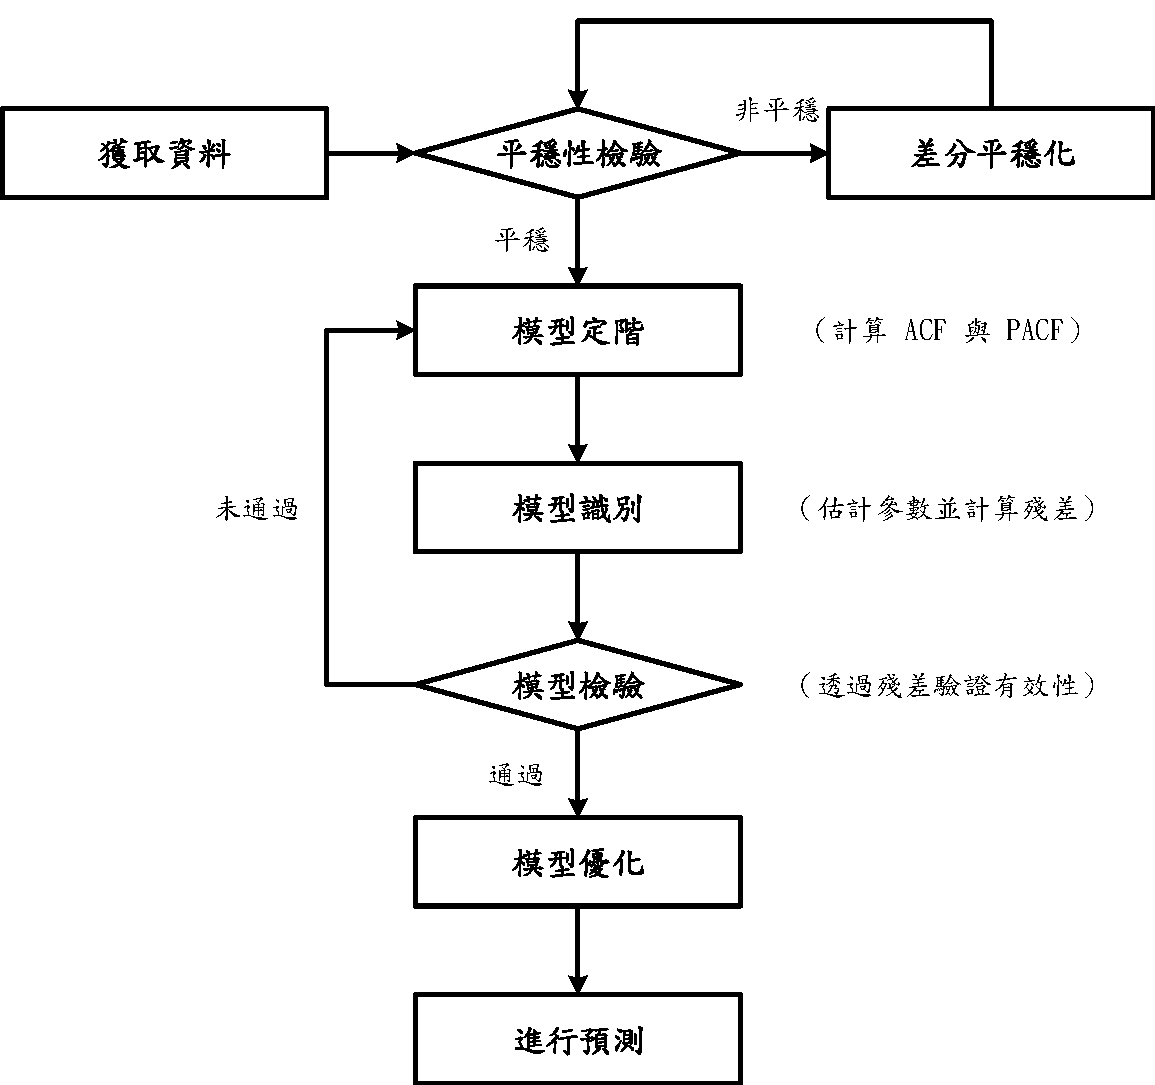
\includegraphics[width=0.84\textwidth]{Time Series Model Flow}
  \caption{時間序列預測建模流程}
  \label{figure: Time Series Model Flow}
\end{figure}

\subsection{支持向量迴歸建模流程}

支持向量迴歸模型建模流程如圖 \ref{figure: Support Vector Regression Flow} 所示,在取得時間序列資料後,將資料集合拆分為訓練集合與測試集合,選定核函數後進行模型訓練,使用測試集合進行評價並選出最適模型進行時間序列預測。

\begin{figure}[htbp]
  \centering
  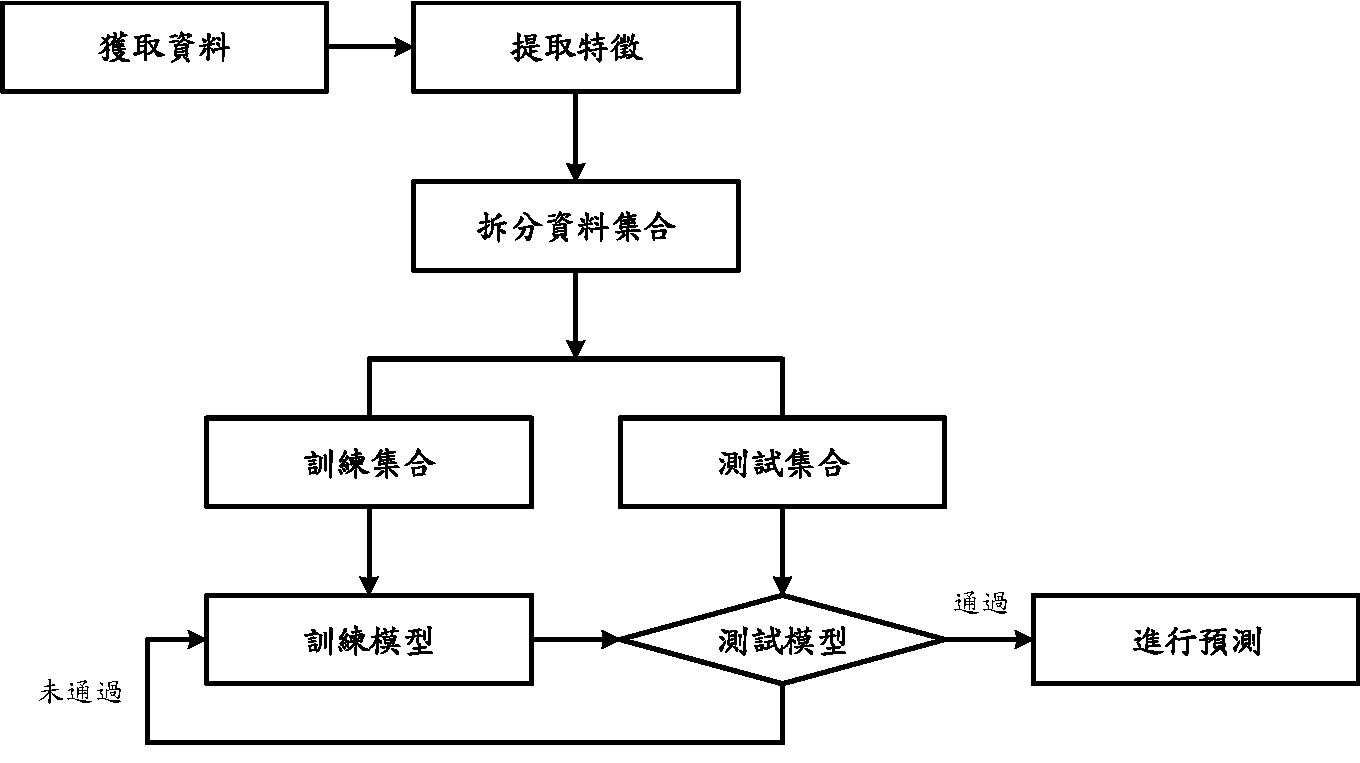
\includegraphics[width=\textwidth]{Support Vector Regression Model Flow}
  \caption{支持向量迴歸建模流程}
  \label{figure: Support Vector Regression Flow}
\end{figure}

\subsection{組合預測模型建模流程}

常見的組合預測模型是將預測的結果進行線性組合,根據加權方式可以再分為採用等權的簡單平均組合以及變動權重組合,前者簡潔較易於計算但無法有效突出不同模型的優勢,後者則需要嘗試不同組合來尋找最佳的權重分配;小波分解則是將原始時間序列進行解構,根據分解後各分量的特性分別採取較佳的預測方法後再將結果進行組合,組合時不需進行權重的分配。本文將採用下述的兩種組合預測模型:

\begin{itemize}
  \item \textbf{一般等權組合預測模型}
    \begin{equation}\label{equation: Normal Combine Model}
      \hat{y(t)} = \frac{1}{2} \hat{y}_{ARIMA} (t) + \frac{1}{2} \hat{y}_{SVR} (t)
    \end{equation}
  \item \textbf{小波分解組合預測模型}
    \begin{equation}\label{equation: Wavelet Combine Model}
      \hat{y(t)} = \hat{A}_{2} (t) + \hat{D}_{1} (t) + \hat{D}_{2} (t)
    \end{equation}
\end{itemize}

上述組合預測模型的建模流程分別如圖 \ref{figure: Linear Combine Model Flow} 和圖 \ref{figure: Wavelet Combine Model Flow} 所示。一般等權組合預測模型即為分別使用單一預測模型進行預測後,將預測結果使用同樣的權重進行線性組合;小波分解組合預測模型則需先將時間序列透過離散小波轉換分解為高頻部分(細節分量)與低頻部分(近似分量),並分別採用 ARIMA 模型預測與 SVR 模型預測,再將預測結果進行整合。

\begin{figure}[htbp]
  \centering
  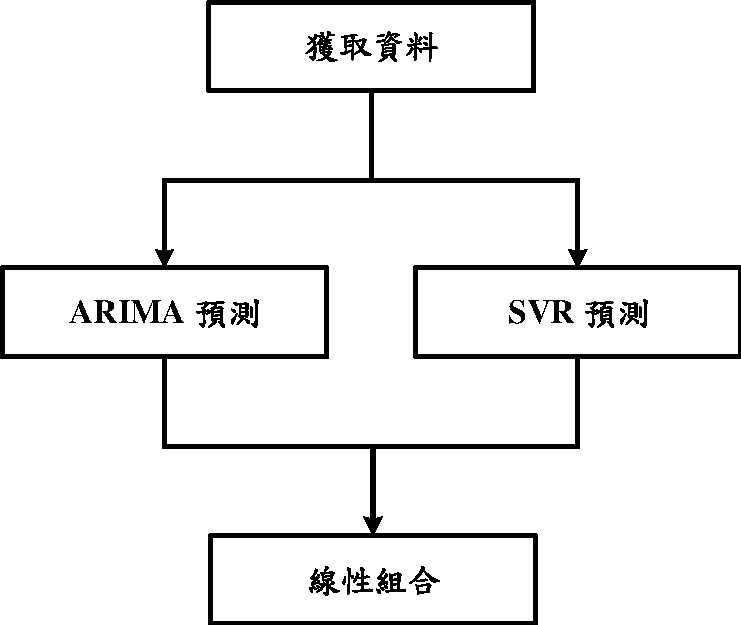
\includegraphics[width=0.55\textwidth]{Linear Combine Model Flow}
  \caption[一般等權組合預測模型建模流程]{一般等權組合預測模型建模流程}
  \label{figure: Linear Combine Model Flow}
\end{figure}

\begin{figure}[htbp]
  \centering
  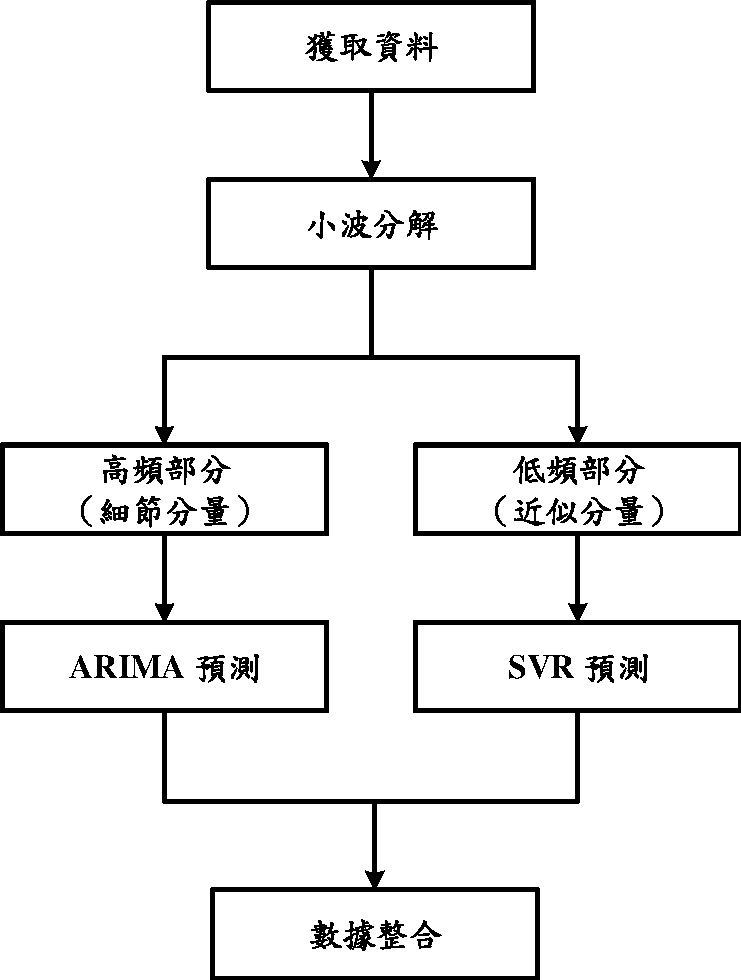
\includegraphics[width=0.55\textwidth]{Wavelet Combine Model Flow}
  \caption[小波分解組合預測模型建模流程]{小波分解組合預測模型建模流程}
  \label{figure: Wavelet Combine Model Flow}
\end{figure}

\section{虛擬電廠收益分析}

\subsection{虛擬電廠結構概述}

本文虛擬電廠結構(Virtual Power Plant, VPP)如圖 \ref{figure: Virtual Power Plant Model} 所示,由風力電場(Wind Farm, WF)、電動汽車(Electric Vehicle, EV)組成,分別透過發電與儲能來參與電力市場(Electric Market, EM)的日前市場調度。

\begin{figure}[htbp]
  \centering
  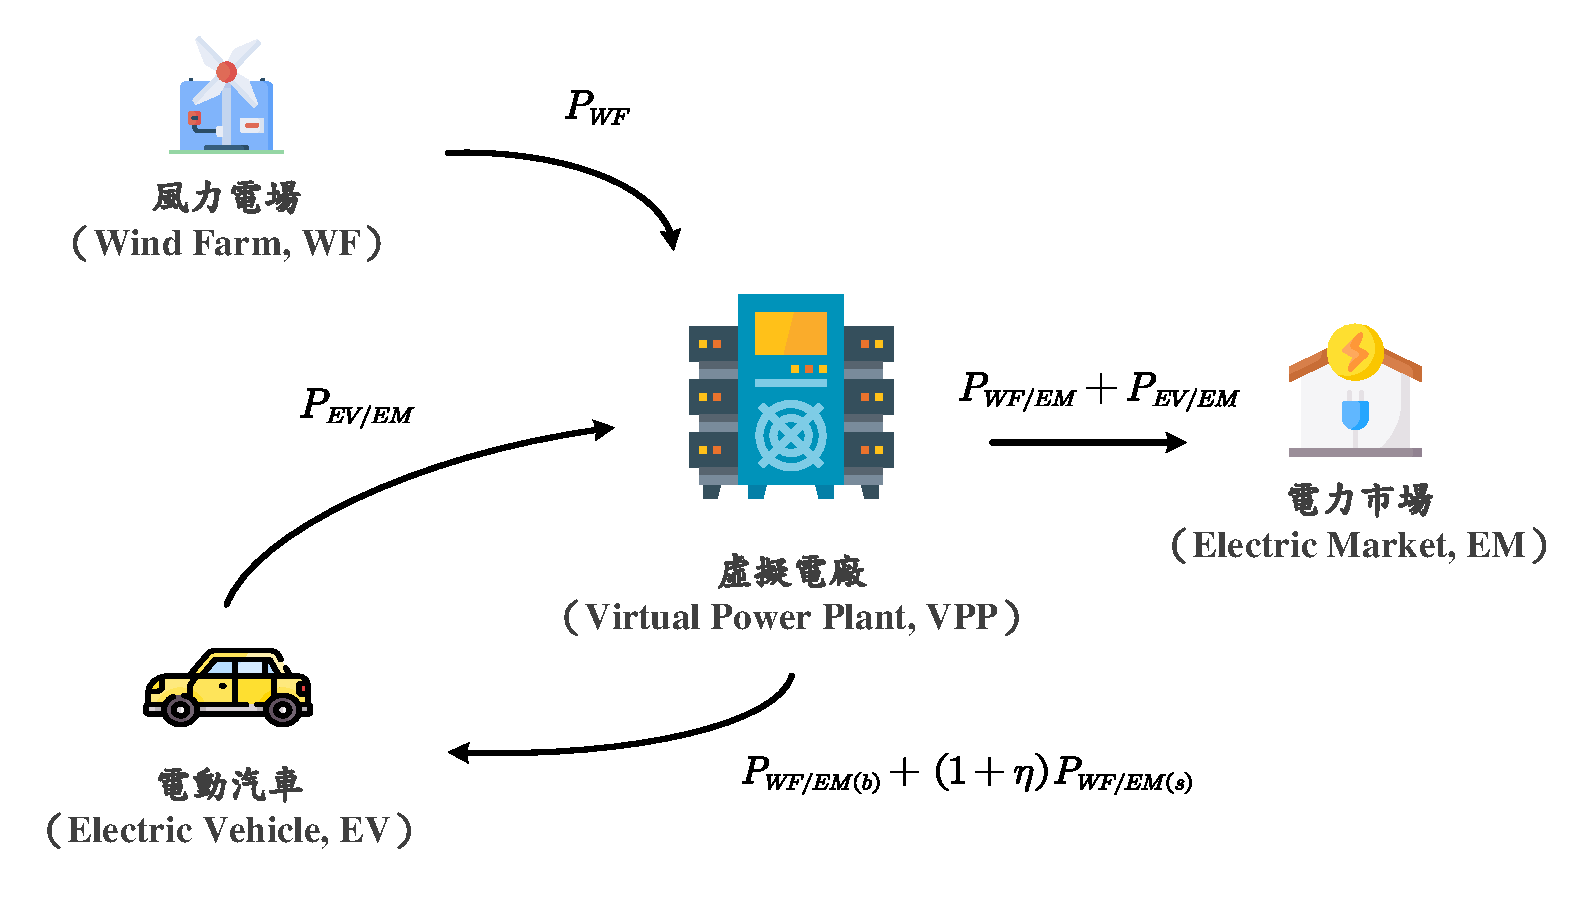
\includegraphics[width=0.8\textwidth]{Virtual Power Plant Model}
  \caption{整合風力電場與電動汽車的虛擬電廠模型}
  \label{figure: Virtual Power Plant Model}
\end{figure}

在日前市場中,電力交易會在前一天完成並在當天公告交易資訊,最後在日前市場關閉後確定隔天的發電數量,發電業者需要簽約保證提供確定的發電數量,若提供的發電數量與確定的發電數量存在偏差,則需要進行賠償。亦即虛擬電廠必須在第 $(t - 1)$ 日提交價格資訊,並保證在第 $t$ 日的每個時段提供一定的電力;在這樣的狀況下,風力電場需要在 $(t - 1)$ 日根據天氣資訊預估發電數量,並在給出第 $t$ 日願意參與虛擬電廠的電動汽車後,決定最佳儲存容量來在日前市場中提出最有利的競標價格。

除此之外,由於參與儲能後會增加電動汽車電池的充電放電次數導致電池壽命減少,因此需要對電動汽車車主進行補償以促進其進行儲能來參與虛擬電廠的動機。但參與虛擬電廠的電動汽車無法如同傳統儲能設備那般計算運轉成本,本文中並不採用直接給予金錢的補償支付,而是無償地向電動汽車提供充電,雖然減少了向電網供電的部分收入,但能夠將電力儲存於電動汽車來降低虛擬電廠的電力波動,整體而言卻能夠獲得更大收益。

\subsection{風力電場等效模型}

若已知特定風力機組 $M$ 的額定功率曲線,則可以透過某一時刻 $t$ 的風速資料 $v(t)$ 確定該時刻所對應的風力機組出力情況,如方程式 \eqref{equation: Wine Turbine Power} 所示。

\begin{equation}\label{equation: Wine Turbine Power}
  P_{wt, M} (t) = P_{wt, M} (v (t))
\end{equation}

假定一風力電場(Wind Farm)內設置有風力發電機組 $M_{1}, M_{2}, \cdots, M_{k}$,則在當天某一時刻 $t$ 的預測發電總量可以表示如方程式 \eqref{equation: Wind Farm Power} 所示。

\begin{equation}\label{equation: Wind Farm Power}
  P_{WF}(t) = \sum_{i = 1}^{k} P_{wt, Mi} (t)
\end{equation}

在本文的模擬情況中,預測風速資料將以每一小時作為時間間隔,為了方便進行建模運算,最終將以向量形式表示在時間內該風力電場不同單位時刻的預測發電總量,用以參與電力市場作為日前市場的投標資訊,如方程式 \eqref{equation: Wind Farm Power Vector} 所示。

\begin{equation}\label{equation: Wind Farm Power Vector}
  \boldsymbol{P_{WF}} = [  P_{WF}(1) P_{WF}(2) P_{WF}(3) \cdots P_{WF}(N) ]^{\top}
\end{equation}

\subsection{電動汽車等效模型}

電動汽車透過儲存電能到電池中來參與虛擬電廠的電力市場交易,對於每一輛電動汽車 $V$ 而言都有其對應的儲存容量,由於電動汽車電池壽命會受到放電深度(Depth of Discharge)影響,進而影響電動汽車駕駛的電力儲存偏好,因此可以透過放電深度 $\text{DoD}$ 與電動汽車額定容量 $E$ 來表示其儲存容量,如方程式 \eqref{equation: Electriv Vehicle Power} 所示。

\begin{equation}\label{equation: Electriv Vehicle Power}
  S_{V} (t) = \text{DoD} \times E
\end{equation}

假定一電動汽車(Electric Vehicle)集合中設置有電動汽車 $V_{1}, V_{2}, \cdots, V_{k}$,則在當天某一時刻 $t$ 的儲存容量總量可以表示如方程式 \eqref{equation: Electriv Vehicle Set Power} 所示。

\begin{equation}\label{equation: Electriv Vehicle Set Power}
  S_{EV}(t) = \sum_{i = 1}^{k} S_{Vi} (t)
\end{equation}

在本文的模擬情況中,為配合以每一小時作為時間間隔的預測風速資料進行建模運算,同樣將以向量形式表示在時間內所有電動汽車在不同單位時刻的儲存容量總量,如方程式 \eqref{equation: Electric Vehicle Power Vector} 所示。

\begin{equation}\label{equation: Electric Vehicle Power Vector}
  \boldsymbol{S_{EV}} = [  S_{EV}(1) S_{EV}(2) S_{EV}(3) \cdots S_{EV}(N) ]^{\top}
\end{equation}

\subsection{電力市場收益模型}

\subsubsection{日前市場調度}

根據前述的虛擬電廠架構,本文將根據風力電場的預測發電數量,調度電動汽車進行儲存能量來參與電力市場交易,並透過規劃求解虛擬電廠的最大收益,其最佳化模型可由方程式 \eqref{equation: Virual Power Plant Profit Model} 表示。

\begin{subequations}\label{equation: Virual Power Plant Profit Model}
  \begin{alignat}{2}
    \max        \qquad & \sum_{t = 1}^{N} p_{e}(t) [P_{WF/EM}(t) + P_{EV/EM}(t)]      \label{subequation: Virual Power Plant Profit Model 1} \\
    \text{s.t.} \qquad & P_{WF/EM}(t) + P_{WF/EV(b)}(t) + (1 + \eta)P_{WF/EV(s)}(t) = P_{WF}(t) \label{subequation: Virual Power Plant Profit Model 2} \\
                       & \sum_{i=1}^{t-1} \left[ P_{WF/EV(s)}(i) - P_{EV/EM}(i) \right] + P_{WF/EV(s)}(t) \leq P_{ST}(n)                    \label{subequation: Virual Power Plant Profit Model 3} \\
                       & \sum_{i=1}^{t-1} \left[ P_{WF/EV(s)}(i) - P_{EV/EM}(i) \right] - P_{EV/EM}(t) \geq 0                       \label{subequation: Virual Power Plant Profit Model 4} \\
                       & P_{WF/EV(b)}(t) \geq \sigma P_{ST}(n)                         \label{subequation: Virual Power Plant Profit Model 5} \\
                       & 0 \leq P_{ST}(n) + P_{WF/EV(b)}(t) \leq S_{EV}(t)             \label{subequation: Virual Power Plant Profit Model 6} \\
                       & P_{WF/EM}(t), P_{WF/EV(s)}(t),  P_{WF/EV(b)}(t),P_{EV/EM}(t) \geq 0                 \label{subequation: Virual Power Plant Profit Model 7}      
  \end{alignat}
\end{subequations}

其中,$p_{e} (t)$ 為虛擬電廠在電力交易市場中的販售電力價格;$P_{WF/EM}(t)$ 為風力電場輸送至電力交易市場中進行販售的電力數量;$P_{WF/EV(s)}(t)$ 為風力電場輸送至電動汽車電池中進行儲存的電力數量;$P_{WF/EV(b)}(t)$ 為風力電場輸送至電動汽車電池中作為補償的電力數量;$P_{EV/EM}(t)$ 為電動汽車輸送至電力交易市場中進行販售的電力數量;$P_{ST}(t)$ 為虛擬電廠需要的電力儲存容量;$\eta$ 為電動汽車電池在充放電過程的能源轉換效率。

% 目標函數說明
式 \eqref{subequation: Virual Power Plant Profit Model 1} 為目標函數,為使電動汽車與風力電場參與虛擬電廠進行電力市場交易的收益最大,其中虛擬電廠販售電力收入可以表示為虛擬電廠販售給電網的電力價格 $p_{e} (t)$ 個別和虛擬電廠傳輸到電網的電力數量 $P_{WF/EM}(t)$ 與電動汽車傳輸到電網的電力數量 $P_{EV/EM}(t)$ 乘積的總和。

% 限制條件說明
式 \eqref{subequation: Virual Power Plant Profit Model 2} 為限制條件,表示風力電場在 $t$ 時刻的預測發電數量 $P_{WF/EM}(t)$ 可以分配 $P_{WF/EM}(t)$ 輸送至電力交易市場中進行販售、$P_{WF/EV(b)}(t)$ 輸送至電動汽車電池中作為補償、$P_{WF/EV(s)}(t)$ 輸送至電動汽車電池中進行儲存,其中考慮了電動汽車電池在充放電過程中存在能源轉換耗損,每一單位的電力數量在充放電時會損失 $\eta$ 單位的電力數量。

式 \eqref{subequation: Virual Power Plant Profit Model 3} 為限制條件,表示在 $t$ 時刻的電動汽車電池過去時刻所累積的(現在所擁有的)儲存電量 $\sum_{i=1}^{t-1} \left[ P_{WF/EV(s)}(i) - P_{EV/EM}(i) \right]$ 與該時刻欲存入的儲存電量 $P_{WF/EV(s)}(t)$ 不得超過電動汽車的可用儲存容量 $P_{ST}(t)$。

式 \eqref{subequation: Virual Power Plant Profit Model 4} 為限制條件,表示在 $t$ 時刻的電動汽車電池能夠輸送至電力交易市場中進行販售的電力數量 $P_{EV/EM}(t)$ 不得超過電動汽車電池過去時刻所累積的(現在所擁有的)儲存電量 $\sum_{i=1}^{t-1} \left[ P_{WF/EV(s)}(i) - P_{EV/EM}(i) \right]$。

式 \eqref{subequation: Virual Power Plant Profit Model 5} 為限制條件,表示風力電場輸送至電動汽車電池中作為補償的電力數量 $P_{WF/EV(b)}(t)$
 需大於虛擬電廠需要的儲存容量 $P_{ST}(t)$ 的一定比例 $\sigma$。

式 \eqref{subequation: Virual Power Plant Profit Model 6} 為限制條件,表示在 $t$ 時刻虛擬電廠需要的儲存容量 $P_{ST}(t)$ 與風力電場輸送至電動汽車電池中作為補償的電力數量 $P_{WF/EV(b)}(t)$ 必須小於所有電動汽車在該時刻的儲存容量總量 $S_{EV}(t)$。

式 \eqref{subequation: Virual Power Plant Profit Model 7} 為非負限制式,表示在任一時刻的電力傳輸過程中,風力電場輸送至電力交易市場中進行販售的電力數量 $P_{WF/EM}(t)$、風力電場輸送至電動汽車電池中進行儲存的電力數量 $P_{WF/EV(s)}(t)$、風力電場輸送至電動汽車電池中作為補償的電力數量 $P_{WF/EV(b)}(t)$ 和 電動汽車輸送至電力交易市場中進行販售的電力數量 $P_{EV/EM}(t)$ 需滿足本文所提出之虛擬電廠架構的傳輸方向。

\subsubsection{模型預測控制}

模型預測控制需要在移動時域下進行規劃,因此在參與電力市場交易時需要在每一時刻更新其供電計劃。因此最佳化模型需要修正如方程式 \eqref{equation: Virual Power Plant Profit MPC Model} 所示。

\begin{subequations}\label{equation: Virual Power Plant Profit MPC Model}
  \begin{alignat}{2}
    \max        \qquad & \sum_{t = 1}^{N} p_{e}(t) [P_{WF/EM}(t) + P_{EV/EM}(t)]      \label{subequation: Virual Power Plant Profit MPC Model 1} \\
    \text{s.t.} \qquad & P_{WF/EM}'(t) + P_{WF/EV(b)}'(t) + (1 + \eta)P_{WF/EV(s)}'(t) = P_{WF}'(t) \label{subequation: Virual Power Plant Profit MPC Model 2} \\
                       & \sum_{i=1}^{t-1} \left[ P_{WF/EV(s)}(i) - P_{EV/EM}(i) \right] + P_{WF/EV(s)}(t) \leq P_{ST}(n)                    \label{subequation: Virual Power Plant Profit MPC Model 3} \\
                       & \sum_{i=1}^{t-1} \left[ P_{WF/EV(s)}(i) - P_{EV/EM}(i) \right] - P_{EV/EM}(t) \geq 0                       \label{subequation: Virual Power Plant Profit MPC Model 4} \\
                       & P_{WF/EV(b)}(t) \geq \sigma P_{ST}(n)                         \label{subequation: Virual Power Plant Profit MPC Model 5} \\
                       & 0 \leq P_{ST}(n) + P_{WF/EV(b)}(t) \leq S_{EV}(t)             \label{subequation: Virual Power Plant Profit MPC Model 6} \\
                       & P_{WF/EM}(t), P_{WF/EV(s)}(t),  P_{WF/EV(b)}(t),P_{EV/EM}(t) \geq 0                 \label{subequation: Virual Power Plant Profit MPC Model 7}      
  \end{alignat}
\end{subequations}

其中,$p_{e} (t)$ 為虛擬電廠在電力交易市場中的販售電力價格;$P_{WF/EM}'(t)$ 為風力電場輸送至電力交易市場中進行販售的電力數量;$P_{WF/EV(s)}'(t)$ 為風力電場輸送至電動汽車電池中進行儲存的電力數量;$P_{WF/EV(b)}'(t)$ 為風力電場輸送至電動汽車電池中作為補償的電力數量;$P_{EV/EM}'(t)$ 為電動汽車輸送至電力交易市場中進行販售的電力數量;$P_{ST}'(t)$ 為虛擬電廠所需要的電力儲存容量;$\eta$ 為電動汽車電池在充放電過程的能源轉換效率。

% 目標函數說明
式 \eqref{subequation: Virual Power Plant Profit MPC Model 1} 為目標函數,為使電動汽車與風力電場參與虛擬電廠進行電力市場交易的收益最大,其中虛擬電廠販售電力收入可以表示為虛擬電廠販售給電網的電力價格 $p_{e} (t)$ 個別和虛擬電廠傳輸到電網的電力數量 $P_{WF/EM}(t)$ 與電動汽車傳輸到電網的電力數量 $P_{EV/EM}(t)$ 乘積的總和。

% 限制條件說明
式 \eqref{subequation: Virual Power Plant Profit MPC Model 2} 為限制條件,表示風力電場在 $t$ 時刻更新後的預測發電數量 $P_{WF/EM}'(t)$ 可以分配 $P_{WF/EM}'(t)$ 輸送至電力交易市場中進行販售、$P_{WF/EV(b)}'(t)$ 輸送至電動汽車電池中作為補償、$P_{WF/EV(s)}'(t)$ 輸送至電動汽車電池中進行儲存,其中考慮了電動汽車電池在充放電過程中存在能源轉換耗損,每一單位的電力數量在充放電時會損失 $\eta$ 單位的電力數量。

式 \eqref{subequation: Virual Power Plant Profit MPC Model 3} 為限制條件,表示在 $t$ 時刻更新後的電動汽車電池過去時刻所累積的(現在所擁有的)儲存電量 $\sum_{i=1}^{t-1} \left[ P_{WF/EV(s)}(i) - P_{EV/EM}(i) \right]$ 與該時刻欲存入的儲存電量 $P_{WF/EV(s)}(t)$ 不得超過電動汽車的可用儲存容量 $P_{ST}(t)$。

式 \eqref{subequation: Virual Power Plant Profit MPC Model 4} 為限制條件,表示在 $t$ 時刻的電動汽車電池能夠輸送至電力交易市場中進行販售的電力數量 $P_{EV/EM}(t)$ 不得超過電動汽車電池過去時刻所累積的(現在所擁有的)儲存電量 $\sum_{i=1}^{t-1} \left[ P_{WF/EV(s)}(i) - P_{EV/EM}(i) \right]$。

式 \eqref{subequation: Virual Power Plant Profit MPC Model 5} 為限制條件,表示風力電場輸送至電動汽車電池中作為補償的電力數量 $P_{WF/EV(b)}(t)$
 需大於虛擬電廠需要的儲存容量 $P_{ST}(t)$ 的一定比例 $\sigma$。

式 \eqref{subequation: Virual Power Plant Profit MPC Model 6} 為限制條件,表示在 $t$ 時刻虛擬電廠需要的儲存容量 $P_{ST}(t)$ 與風力電場輸送至電動汽車電池中作為補償的電力數量 $P_{WF/EV(b)}(t)$ 必須小於所有電動汽車在該時刻的儲存容量總量 $S_{EV}(t)$。

式 \eqref{subequation: Virual Power Plant Profit MPC Model 7} 為非負限制式,表示在任一時刻的電力傳輸過程中,風力電場輸送至電力交易市場中進行販售的電力數量 $P_{WF/EM}(t)$、風力電場輸送至電動汽車電池中進行儲存的電力數量 $P_{WF/EV(s)}(t)$、風力電場輸送至電動汽車電池中作為補償的電力數量 $P_{WF/EV(b)}(t)$ 和 電動汽車輸送至電力交易市場中進行販售的電力數量 $P_{EV/EM}(t)$ 需滿足本文所提出之虛擬電廠架構的傳輸方向。

\subsection{預測控制求解流程}

模型預測控制求解流程如圖 \ref{figure: Model Predictive Control Flow} 所示,在取得當前時刻 $t$ 的系統資訊後,求解預測時域內的最佳化收益結果,若未完成控制時域內之預測,求解控制變數 $U(t)$ 並使用下一時段之控制變數 $u(t + 1)$ 進行系統調度,反覆進行以求得最佳收益。

\begin{figure}[htbp]
  \centering
  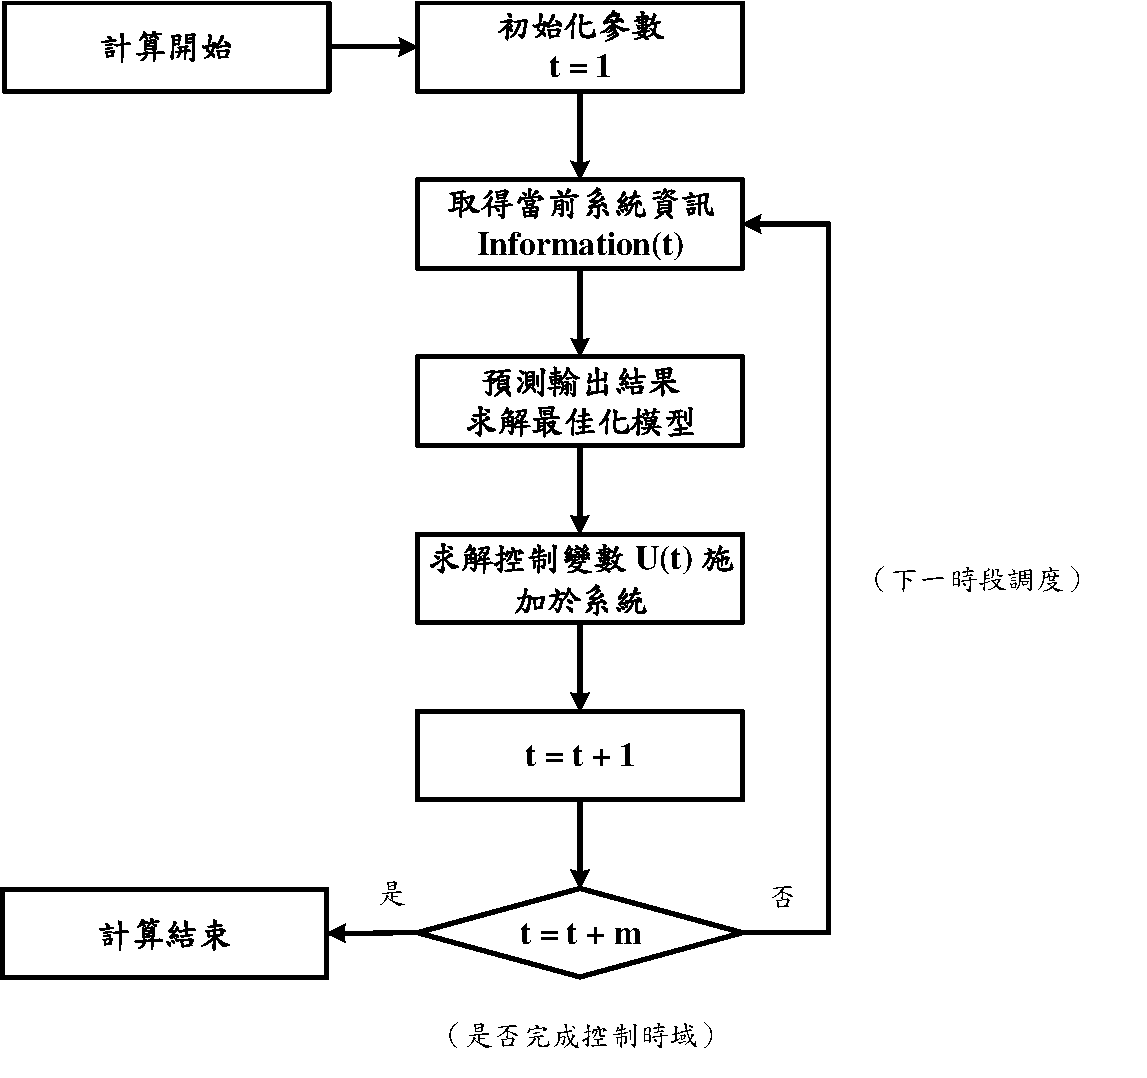
\includegraphics[width=0.85\textwidth]{Model Predictive Control Flow}
  \caption{模型預測控制求解流程}
  \label{figure: Model Predictive Control Flow}
\end{figure}

\section{小結}

本章說明了短期風速預測中時間序列整合自迴歸移動平均模型、支持向量迴歸與使用離散小波進行分解的組合預測模型建模流程,以及收益分析中風力電場與電動汽車等效模型、虛擬電廠最佳化收益模型以及考慮了移動時域的模型預測控制求解流程。透過模型預測可以使得虛擬電廠在參與電力市場交易時,在有限時域中使用前一時刻的系統資訊進行模型規劃以求得最大利潤,在下一章節中將實際使用我國\uline{澎湖}地區的風速資料進行發電預測並進行收益分析。
